\section{Introduction}

\begin{frame}[c]{Motivation}
    \begin{columns}
        \column{0.55\textwidth}
    \begin{figure}
        \centering
    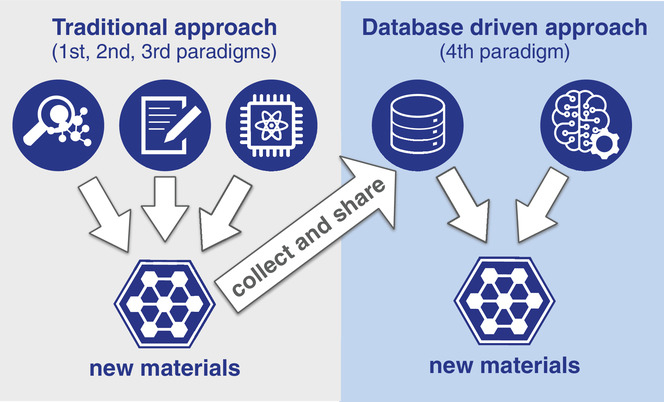
\includegraphics[height=0.6\textheight]{data_driven}
    \caption{
    Image Source: \cite{himanen_datadriven_2019}
    }
    \end{figure}
    \column{0.4\textwidth}
    \large
    \gls{ML} models are increasingly used in screening steps for materials discovery and property prediction \cite{saal_machine_2020, luo_mof_2022, choudhary_recent_2022}.
    Yet, \textbf{most previous research is not available in a machine-readable format}.
\end{columns}
\end{frame}

\begin{frame}[c]{Scientific Questions}
    \large
    % The goals of this work are threefold:
    There are three main questions this work aims to answer:
    \begin{enumerate}[<+(1)->]
        \item Can I demonstrate high accuracy in zero-shot automated information extraction from scientific literature using open-access \glspl{LLM}?
        \item How do currently available open-access \glspl{LLM} compare for this task?
        \item How easy is it to fine-tune open-access \glspl{LLM} for this task? How much does the accuracy increase from fine-tuning?
    \end{enumerate}
    \pause
    \vfill
    While we're at it, create an automated pipeline for information extraction from unstructured text.
\end{frame}
